% !TEX TS-program = pdflatex
% !TEX encoding = UTF-8 Unicode

% This file is a template using the "beamer" package to create slides for a talk or presentation
% - Talk at a conference/colloquium.
% - Talk length is about 20min.
% - Style is ornate.

% MODIFIED by Jonathan Kew, 2008-07-06
% The header comments and encoding in this file were modified for inclusion with TeXworks.
% The content is otherwise unchanged from the original distributed with the beamer package.

\documentclass{beamer}


% Copyright 2004 by Till Tantau <tantau@users.sourceforge.net>.
%
% In principle, this file can be redistributed and/or modified under
% the terms of the GNU Public License, version 2.
%
% However, this file is supposed to be a template to be modified
% for your own needs. For this reason, if you use this file as a
% template and not specifically distribute it as part of a another
% package/program, I grant the extra permission to freely copy and
% modify this file as you see fit and even to delete this copyright
% notice. 


\mode<presentation>
{
  \usetheme{Warsaw}
  % or ...

  \setbeamercovered{transparent}
  % or whatever (possibly just delete it)
}


\usepackage[english,spanish]{babel}


\usepackage[utf8]{inputenc}
% or whatever

\usepackage{graphicx}
\graphicspath{ {img/} }


\usepackage{times}
\usepackage[T1]{fontenc}
% Or whatever. Note that the encoding and the font should match. If T1
% does not look nice, try deleting the line with the fontenc.


\title[GaN Etching] % (optional, use only with long paper titles)
{Gallium Nitride: Dry Etching and Wet Etching}

%\subtitle
%{Include Only If Paper Has a Subtitle}

\author[A. Di Donato] % (optional, use only with lots of authors)
{Andrés~Di Donato\inst{1}}
% - Give the names in the same order as the appear in the paper.
% - Use the \inst{?} command only if the authors have different
%   affiliation.

\institute[CNEA] % (optional, but mostly needed)
{
  \inst{1}%
  Departamento de Micro y Nano Tecnología\\
  Comisión Nacional de Energía Atómica
}
% - Use the \inst command only if there are several affiliations.
% - Keep it simple, no one is interested in your street address.

\date[MDDSC 2019] % (optional, should be abbreviation of conference name)
{Materiales and Devices: their Design, Simulation and Characterization, UNSAM, 2019}
% - Either use conference name or its abbreviation.
% - Not really informative to the audience, more for people (including
%   yourself) who are reading the slides online

\subject{GaN Etching}
% This is only inserted into the PDF information catalog. Can be left
% out. 



% If you have a file called "university-logo-filename.xxx", where xxx
% is a graphic format that can be processed by latex or pdflatex,
% resp., then you can add a logo as follows:

% \pgfdeclareimage[height=0.5cm]{university-logo}{university-logo-filename}
% \logo{\pgfuseimage{university-logo}}



% Delete this, if you do not want the table of contents to pop up at
% the beginning of each subsection:
\AtBeginSubsection[]
{
  \begin{frame}<beamer>{Outline}
%\fontsize{10pt}{7.2}\selectfont
    \tableofcontents[currentsection,currentsubsection]
  \end{frame}
}


% If you wish to uncover everything in a step-wise fashion, uncomment
% the following command: 

%\beamerdefaultoverlayspecification{<+->}


\begin{document}

\begin{frame}
  \titlepage
\end{frame}

\begin{frame}{Outline}
  \tableofcontents
  % You might wish to add the option [pausesections]
\end{frame}


% Structuring a talk is a difficult task and the following structure
% may not be suitable. Here are some rules that apply for this
% solution: 

% - Exactly two or three sections (other than the summary).
% - At *most* three subsections per section.
% - Talk about 30s to 2min per frame. So there should be between about
%   15 and 30 frames, all told.

% - A conference audience is likely to know very little of what you
%   are going to talk about. So *simplify*!
% - In a 20min talk, getting the main ideas across is hard
%   enough. Leave out details, even if it means being less precise than
%   you think necessary.
% - If you omit details that are vital to the proof/implementation,
%   just say so once. Everybody will be happy with that.

\section{Motivation}
\subsection{Etching necessity}

\begin{frame}{Etching necessity}
Etching is very important for defining devices. Some classical examples are:


      \pause
    \begin{itemize}
    \item
      Etching for further formation of ohmic contacts
      \pause
    \item    
      Mesa-etch isolation
    \end{itemize}
\end{frame}


\subsection{Important etching parameters}
  
\begin{frame}{Etching parameters}
Some etching aspects are specially important in semiconductor production\dots

   Some of them are:
      \pause
    \begin{itemize}
    \item
 	Etch rate
      \pause
    \item
 	Selectivity with PHR and dielectrics
      \pause
    \item
 	Isotropy control
      \pause
    \item
	Repeatibility
      \pause
    \item
	Cost
      \pause
    \item
	Equipment required
    \end{itemize}
\end{frame}

\subsection{Comparison between Dry and Wet Etching}

\begin{center}
    \begin{tabular}{ | l | l |l|}
    \hline
     & Dry Etching & Wet etching  \\ \hline
    Etch rate & Lower & Higher  
 \\ \hline

    Isotropy control & Very good & Poor \\ \hline
    Repeatability  & Excellent & Good 
   \\ \hline
Cost  & Higher (gases + electricity) & Lower
   \\ \hline
Equipment required  & Complex (Vaccuum,  MFCs) & Very simple 
   \\ \hline
Sample damage  & Higher & Lower 
   \\ \hline
    \end{tabular}
\end{center}



\section{Dry etching techniques}

\subsection{RIE}
\begin{frame}{RIE - Reactive ion etching}

    \begin{itemize}
    \item
	Combination of Phsyical and chemical etching
      \pause
    \item
 	Physical = non-reactive ions
      \pause
    \item
 	Chemical = reactive ions
\pause
    \item
 	Mostly using $Cl$ based gases por GaN
\end{itemize}

\begin{center}
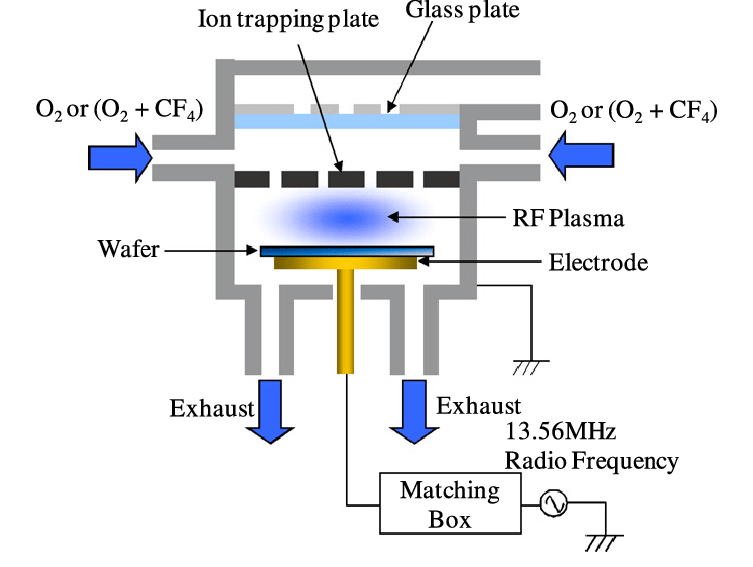
\includegraphics[width=0.7\textwidth]{rie.png}
\end{center}

\end{frame}

\subsection{ICP}
\begin{frame}{ICP RIE - Inductevely Coupled Plasma}

    \begin{itemize}
    \item
	Similar to RIE, but magnetic field generated plasma
      \pause
    \item
	Much denser plasma and consequently higher etch rate
      \pause
    \item
	Tends to be more isotropic
    \item
Possible to combinate with common RIE in same process
\end{itemize}

\begin{center}
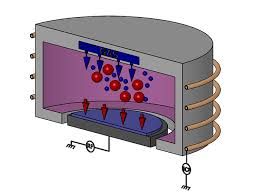
\includegraphics[width=0.5\textwidth]{icp.jpeg}
\end{center}

\end{frame}


\subsection{RIBE}
\begin{frame}{RIBE - Reactive Ion Beam Etching}

Uses an Ion Beam instead of plasma+gases

\begin{center}
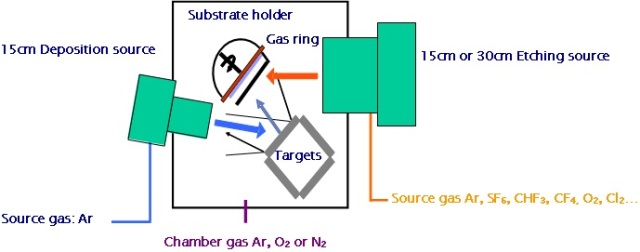
\includegraphics[width=0.9\textwidth]{RIBE.jpg}
\end{center}

\end{frame}

\subsection{ECR Plasma}
\begin{frame}{ECR - Electron Cyclotron Resonance Plasma}

    \begin{itemize}
    \item
    Ultra-Low Pressure and Highest Density Plasma
      \pause
    \item
Plasma distribution and height control
      \pause
    \item
Ion and radical control
    \item
Temperature control
\end{itemize}

\begin{center}
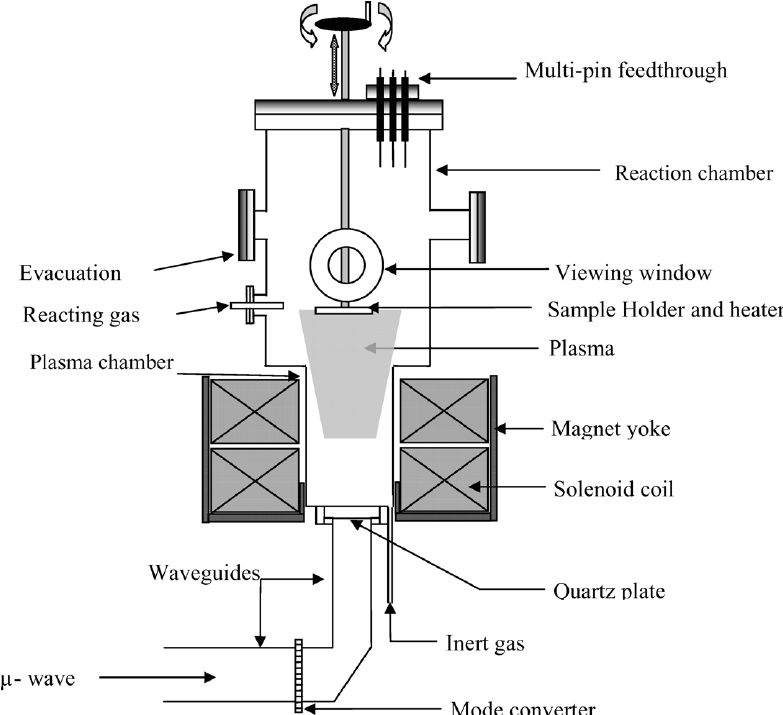
\includegraphics[width=0.4\textwidth]{ECR.png}
\end{center}

\end{frame}


\subsection{Photo Assisted Dry Etching}
\begin{frame}{Photo Assisted Dry Etching}



    \begin{itemize}
    \item
Simulataneous exposure of reactive gas and UV laser radiation
 \pause
    \item
Laser interaction with the surface, bulk and reactants leads to bondbreaking and desortion of reactant.
\pause
    \item
Promising for achieveing damage-free etching
\item
For GaN, HCl with ArF (193nm) laser is typically used
\end{itemize}

\begin{center}
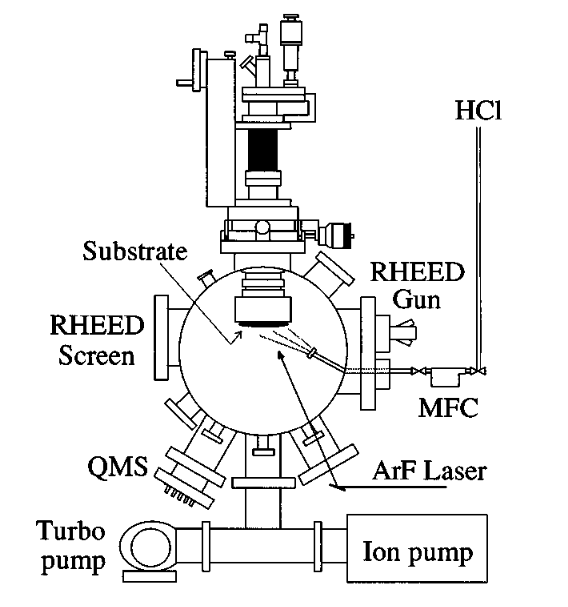
\includegraphics[width=0.3\textwidth]{photo.png}
\end{center}

\end{frame}

\section{Wet etching techniques}

\subsection{Wet Etching with KOH}
\begin{frame}{Wet chemical etching with KOH}

    \begin{itemize}
    \item
Wet chemical etching
 \pause
    \item
Very simple and cheap
    \item
Very smooth surface termination
\end{itemize}
\end{frame}


\subsection{Photo enhanced wet Etching with KOH}
\begin{frame}{UV+KOH}

    \begin{itemize}
    \item
Wet chemical etching
 \pause
    \item
Xenon lamp for UV illumination and KOH solution
    \item
UV is used as cathalyzer

\end{itemize}
\begin{center}
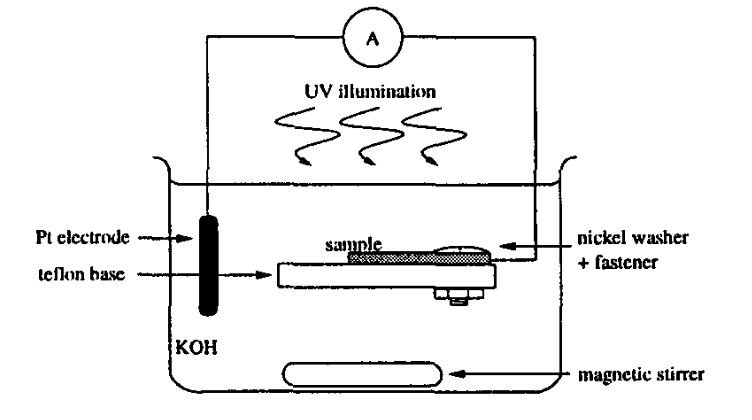
\includegraphics[width=0.8\textwidth]{koh.png}
\end{center}

\end{frame}


\section*{Summary}

\begin{frame}{Summary}

  % Keep the summary *very short*.
  \begin{itemize}
  \item
    \alert{Definition of important etching parameters} will be stated.
  \item
    \alert{General aspects of dry and wetching} will be explained.
  \item
    \alert{Specific Dry and Wet Etching for Gan} techniques will be reviewed, focusing on the ones available at CNEA CAC DMNT. More wet etch techniques are to be studied.
  \end{itemize}
  
  % The following outlook is optional.
  \vskip0pt plus.5fill
  \begin{itemize}
  \item
    Outlook
    \begin{itemize}
    \item
	Get consistent data for comparison
    \item
	Presentation of the informatino and conclussions
    \end{itemize}
  \end{itemize}
\end{frame}



% All of the following is optional and typically not needed. 
\appendix
\section<presentation>*{\appendixname}
\subsection<presentation>*{For Further Reading}

\begin{frame}[allowframebreaks]
  \frametitle<presentation>{For Further Reading}
    
  \begin{thebibliography}{10}
    
%  \beamertemplatebookbibitems
%  % Start with overview books.
%
%  \bibitem{Author1990}
%    A.~Author.
%    \newblock {\em Handbook of Everything}.
%    \newblock Some Press, 1990.
 
    
  \beamertemplatearticlebibitems
  % Followed by interesting articles. Keep the list short. 

  \bibitem{Lee98}
    J.~Lee et al.
    \newblock Dry Etching of GaN and Related Materials:
Comparison of Techniques.
    \newblock {\em IEEE Journal of Selected Topics in Quantum Electronics}, 1998.

  \bibitem{Kinder}
    B.~Kinder and T.~Tansley.
    \newblock A Comparative Study of Photoenhanced Wet
Chemical Etching and Reactive Ion Etching of
GaN Epilayers Grown on Various Substrates
    \newblock {\em Conference on Optoelectronic and Microelectronic Materials and Devices. Proceedings (Cat. No.98EX140)}, 1999.

  \end{thebibliography}
\end{frame}

\end{document}


